\documentclass[a4,11pt]{article}

\usepackage{./exercises}
\usepackage{./macros}
\usepackage{mathtools}
\usepackage{tikz}

\usepackage{graphicx}
\usepackage{ngerman}

\vltitel{Lineare Algebra 2}
\dozent{\small{Christian Haase}}
\assistent{\small{Jan Marten Sevenster}}
\tutoren{\small{%
    Theresa Graeber \\[-1ex] Eva Schinzel}}

\semester{Sommersemester 2023%
  % \raisebox{-10mm}[0pt][0pt]{%
  %   \parbox{0pt}{\includegraphics[width=27mm]{../../2015-ana1-L/Vorlesungsmaterial/ana1QR}}}
}

\DeclareMathOperator{\End}{End}
\DeclareMathOperator{\Span}{span}
% \DeclareMathOperator{\ker}{ker}
\DeclareMathOperator{\im}{im}
\newcommand{\bonusitem}{\item\hspace*{-2.4mm}*\ }


\begin{document}
\vspace*{-17mm}
{
\kopf
}
% \vspace*{-5mm}
% \enlargethispage*{25mm}

\newcounter{chapter}
\ueblatt{12}{ Montag, 17.~Juli 2023 um 10h00}


\begin{aufgabe}[4 Punkte]
Aus lineare algebra eins wissen wir, dass es f"r jede lineare Abbildung $F : V \to W$ des Rangs $r$, Basen $B_V$ und $B_W$ von $V$ und $W$ gibt, sodass die Matrix $M(F)_{B_V}^{B_W}$ links oben eine Einheitsmatrix $E_r$ hat und sonst nur Nullen. 
\begin{enumerate}
\item
Warum impliziert die Existenz dieser Basen nicht die Existenz der Singul"arwertzerlegung von $M$?
\item
Kann mann umgekehrt aus der Singul"arwertzerlegung von $M$ direkt die Existenz der oben beschriebene Basen folgern?
\end{enumerate}
\end{aufgabe}

\begin{aufgabe}[4 Punkte]
Wir betrachten den Graf %$(\{s_1, s_2, s_3, s_4\},\{(s_1, s_2), (s_1, s_3), (s_1, s_4), (s_2, s_3), (s_2, s_4), (s_3, s_1), (s_4, s_1), (s_4, s_3) \})$ 
\[
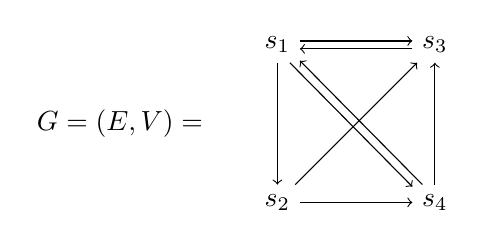
\begin{tikzpicture}
\node at (-2, 1) {$G = (E, V) = $};

\node (s3) at (2,2) {$s_3$};
\node (s4) at (2,0) {$s_4$};
\node (s2) at (0,0) {$s_2$};
\node (s1) at (0,2) {$s_1$};

\draw[->] (s1) -- (s2);
\draw[->] (s1.10) -- (s3.170);
\draw[->] (s1.305) -- (s4.145);

\draw[->] (s2) -- (s3);
\draw[->] (s2) -- (s4);

\draw[->] (s3.190) -- (s1.350);

\draw[->] (s4.125) -- (s1.325);
\draw[->] (s4) -- (s3);
\end{tikzpicture}
\]

Zu diesem Graf konstruieren wir die Matrix $A$ wie beschrieben in der Vorlesung. Wir setzen
\[
A_{ji} = \begin{cases}
1 / \# \{ v \in V \mid v \text{ f"angt in } s_i \text{ an}\}, & \text{falls es ein } v \in V \text{  von } s_i \text{ nach } s_j \text{ existiert}\\
0, & sonst.
\end{cases}
\]

\begin{enumerate}
\item
Verifizieren Sie, dass Eig$(A;1)$ eindimensional ist.
\item
Wir wollen den Pagerank manipulieren, ohne mit den Webmastern f"ur
  die Seiten $s_1$ bis $s_4$ zu reden. Dazu f"ugen wir ein Netz von fake
  Seiten ein, die sich untereinander verlinken und von denen einige
  auf die von uns pr"aferierte Seite $s_2$ verweisen.
  Wie "andert sich der Pagerank?*
 \item
  Durch Zufall lernen wir Webmaster $s_4$ auf der Fachbereichsparty
  kennen. Wir k"onnen sie "uberzeugen, einen Link auf eine unserer
  fake Seiten auf ihre Seite zu stellen. Wie "andert sich der Pagerank?*
\end{enumerate}
 *Sie d"urfen ein Beispiel angeben, das die Situation illustriert, oder eine allgemeine Aussage ableiten und beweisen.
\end{aufgabe}


\begin{aufgabe}[4 Punkte]
Ein Spaziergang der L"ange $\ell \in \N$ in einem Internet $G=(V,E)$ ist
eine Folge von Seiten $v_0, \ldots, v_\ell \in V$ (Wiederholungen
erlaubt), so dass f"ur $i=1, \ldots, \ell$ $(v_{i-1},v_i) \in E$.

Zu einer Matrix $A \in M(n \times n; \R)$ mit nicht-negativen
Eintr"agen k"onnen wir ein Internet auf den Seiten $V = \{ 1, \ldots,
n \}$ definieren: $(i,j) \in E :\Leftrightarrow a_{ij} > 0$.

Zeigen Sie, dass f"ur $i,j \in V$ der $ij$-Eintrag der $\ell$-ten
Potenz $A^\ell$ genau dann positiv ist, wenn es in $G=(V,E)$ einen
Spaziergang der L"ange $\ell$ von $j$ nach $i$ gibt.
  
\end{aufgabe}

\end{document}

%%% Local Variables: 
%%% mode: latex
%%% End: 
